% \documentclass{standalone}
% \input{../tikz_header}

% \begin{document}

 
 
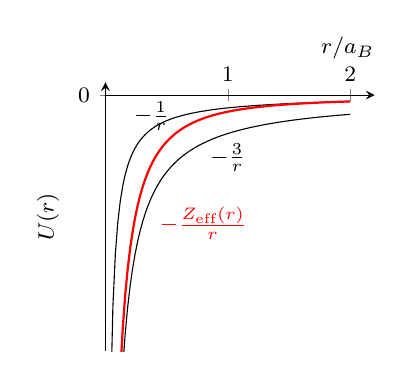
\begin{tikzpicture}[font=\footnotesize]

  \begin{axis}[
    xmin =0,
    xmax = 2.2,
    ymax = 1,
    ymin = -20,
    xlabel =  $r / a_B$ ,
    ylabel =  $U(r)$,
    % ytick = {0,1},
    % xticklabels = { $0$, $L$},
    % yticklabels = { $0$, $L$},
    ytick = {0},
    xtick = {0, 1, 2},
     axis y line = left,
     axis x line = center,
    width = 50mm,
    height=50mm,
    every x tick  label/.style={
      %at={(xticklabel cs:0.9,5pt)},
      anchor=south,
      inner sep=7pt,
  }, 
  x label style={at={(axis description cs:0.9,1.05)},anchor=south},
    ]

    \addplot[domain=0:2, samples =100] {- 1/x };
    \addplot[domain=0:2, samples =100] {- 3/x };
    \node[below] at (1,-3) {$-\frac{3}{r}$};
    \node[left] at (0.6,{-1/0.6}) {$-\frac{1}{r}$};

    % Z_eff from Chap 8, UE 86 in Harris, Modern Physics
    \addplot[red,thick, domain=0:2, samples =100] {- (1/x ) * (7.5 * exp(-1.26*x) - 5.5 *exp(-1.1*x) +1)};
    \node[red] at (0.8, -10) {$- \frac{Z_\textrm{\tiny eff}(r)}{r}$};

\end{axis}
\end{tikzpicture}


%\end{document}


